\documentclass{standalone}

\usepackage{tikz}

\usetikzlibrary{patterns}
\usetikzlibrary{arrows.meta}

\usepackage{bm}

\begin{document}

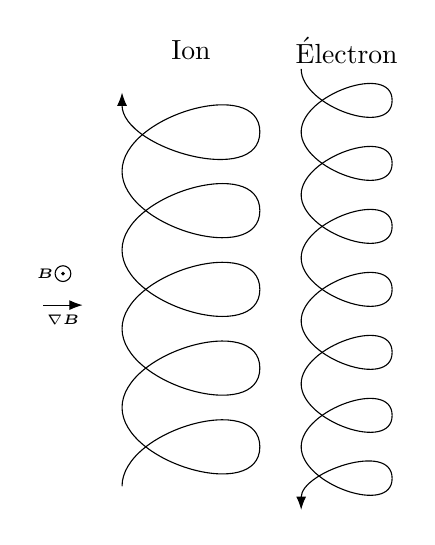
\begin{tikzpicture}

	\def\offsetion{0.5}
	\def\widthion{2*\offsetion}
	\def\heightion{1.75}
	
	\def\offsete{0.4}
	\def\widthe{2*\offsete}
	\def\heighte{0.66*\heightion}

	\def\nion{3}
	\def\ne{5}
	
	\draw[ -{Latex} ] (-1, -0.2) -- (-0.5, -0.2) node[midway, anchor=north] {\tiny \( \nabla\bm{B} \)};
	
	\fill (-0.75, 0.2) circle [radius=0.025];
	\draw (-0.75, 0.2) circle [radius=0.1] node[ anchor=east ] {\tiny \( \bm{B} \)};
	
	\foreach \i in {0, ..., \nion} {
		\draw (0, -\nion/2*\widthion-\widthion+\i*\widthion) to[out=90, in=90]	(\heightion, -\nion/2*\widthion-\widthion+\i*\widthion+\offsetion);
		\draw (\heightion, -\nion/2*\widthion-\widthion+\i*\widthion+\offsetion) to[ out=-90, in=-90 ] (0, -\nion/2*\widthion-\widthion+\i*\widthion+\widthion);
	};
	\draw (0, -\nion/2*\widthion+\nion*\widthion) to[out=90, in=90]	(\heightion, -\nion/2*\widthion+\nion*\widthion+\offsetion);
	\draw[ -{Latex} ] (\heightion, -\nion/2*\widthion+\nion*\widthion+\offsetion) to[ out=-90, in=-90 ] (0, -\nion/2*\widthion+\nion*\widthion+\widthion);
	
	\foreach \i in {0, ..., \ne} {
		\draw (\heightion*1.3, \ne/2*\widthe+\widthe-\i*\widthe) to[out=-90, in=-90] (\heightion*1.3+\heighte, \ne/2*\widthe+\widthe-\i*\widthe-\offsete);
		\draw (\heightion*1.3+\heighte, \ne/2*\widthe+\widthe-\i*\widthe-\offsete) to[out=90, in=90] (\heightion*1.3, \ne/2*\widthe-\i*\widthe);
	}
	\draw (\heightion*1.3, \ne/2*\widthe-\ne*\widthe) to[out=-90, in=-90] (\heightion*1.3+\heighte, \ne/2*\widthe-\ne*\widthe-\offsete);
		\draw[ -{Latex} ] (\heightion*1.3+\heighte, \ne/2*\widthe-\ne*\widthe-\offsete) to[out=90, in=90] (\heightion*1.3, \ne/2*\widthe-\widthe-\ne*\widthe);
		
		\node at (\heightion*1.3+\heighte/2, \ne/2*\widthe+\widthe*1.3) {Électron};
		\node at (\heightion/2, \ne/2*\widthe+\widthe*1.3) {Ion};

\end{tikzpicture}

\end{document}